% 120 x 72 cm. Build: xelatex -jobname=RenalLens_Poster main.tex
\documentclass{article}
\usepackage[paperwidth=120cm,paperheight=72cm,margin=0cm]{geometry}
\usepackage{fontspec,unicode-math,graphicx,tikz,booktabs,array,hyperref}
\setmathfont{texgyretermes-math.otf}
\setmainfont[BoldFont=texgyretermes-bold.otf,ItalicFont=texgyretermes-italic.otf,BoldItalicFont=texgyretermes-bolditalic.otf]{texgyretermes-regular.otf}
\setsansfont[BoldFont=texgyreheros-bold.otf]{texgyreheros-regular.otf}
\definecolor{navy}{HTML}{163E77}
\definecolor{blue}{HTML}{315FAE}
\definecolor{kidney}{HTML}{2163C6}
\definecolor{green}{HTML}{4C9D2F}
\definecolor{red}{HTML}{D82F26}
\definecolor{orange}{HTML}{ED7609}
\definecolor{ink}{HTML}{171717}
\definecolor{muted}{HTML}{50555C}
\definecolor{grayline}{HTML}{B9C1CD}
\hypersetup{colorlinks=true,urlcolor=navy,pdftitle={RenalLens: Beyond the urine test in chronic kidney disease},pdfauthor={BAI Yingdong, CHEN Canyang, LI Jiaheng, PENG Peiyan, ZHAI Junsong, ZHANG Junjie},pdfsubject={DSC5002 C61 Group 65}}
\pagestyle{empty}
\setlength\parindent{0pt}
\newcommand{\sz}[2]{\fontsize{#1}{#2}\selectfont}
\newsavebox{\textfit}
% Every text block has an explicit maximum height, checked at build time.
\newcommand{\content}[5]{%
  \node[anchor=north west,inner sep=0pt,outer sep=0pt] at (#1,-#2) {%
  \sbox{\textfit}{\begin{minipage}[t]{#3cm}\normalfont\rmfamily\raggedright\color{ink}\sz{32}{39}#5\end{minipage}}%
  \ifdim\dimexpr\ht\textfit+\dp\textfit\relax>#4cm
    \PackageError{poster}{Text exceeds block at (#1,#2): \the\dimexpr\ht\textfit+\dp\textfit\relax}{Shorten or move the text.}\fi
  \usebox{\textfit}};
}
\newcommand{\strip}[4]{%
  \fill[blue] (#1,-#2) rectangle ++(#3,-1.25);
  \node[anchor=west,text=white,inner sep=0pt,font=\sffamily\bfseries\sz{32}{36}] at (#1+0.45,-#2-0.625) {#4};
}
\newcommand{\ruleat}[3]{\draw[grayline,line width=1.3pt] (#1,-#2) -- ++(#3,0);}
\begin{document}
\null
\begin{tikzpicture}[remember picture,overlay,x=1cm,y=1cm]
\begin{scope}[shift={(current page.north west)}]
  \fill[white] (0,0) rectangle (120,-72);
  \fill[navy] (0,0) rectangle (120,-9.0);
  \content{2.5}{0.75}{98}{1.2}{{\color{white}\sffamily\bfseries\sz{29}{34}RENALLENS\hspace{1.3cm}DSC5002\hspace{0.5cm}C61 GROUP 65}}
  \content{2.5}{2.25}{99}{3.1}{{\color{white}\bfseries\sz{80}{88}Beyond the urine test in chronic kidney disease}}
  \content{2.5}{5.78}{98}{1.4}{{\color{white}\sz{32}{38}BAI Yingdong, CHEN Canyang, LI Jiaheng, PENG Peiyan, ZHAI Junsong and ZHANG Junjie}}
  \content{2.5}{7.28}{98}{1.1}{{\color{white}\sz{29}{34}City University of Hong Kong}}
  \node[anchor=north east,inner sep=0pt] at (117.5,-1.0) {
\includegraphics[width=13.2cm]{CityUHK_Logo.png}};

  % Left two thirds: question, full approved Figure 1, interpretation.
  \strip{2.5}{10.0}{78.5}{RESEARCH QUESTION AND COHORT}
  \content{2.5}{11.85}{78.5}{1.8}{{\bfseries\sz{40}{46}What can blood measurements add when urine albumin is grade 0?}}
  \content{2.5}{13.75}{78.5}{2.7}{We examined \textbf{250 CKD-labeled records} from the 400-record UCI dataset. Each analysis used its available measurements. We compared kidney markers, hemoglobin and glucose, then examined co-occurring findings.}

  \strip{2.5}{17.0}{78.5}{ANALYSIS FRAMEWORK}
  \node[anchor=north west,inner sep=0pt] at (2.5,-18.4) {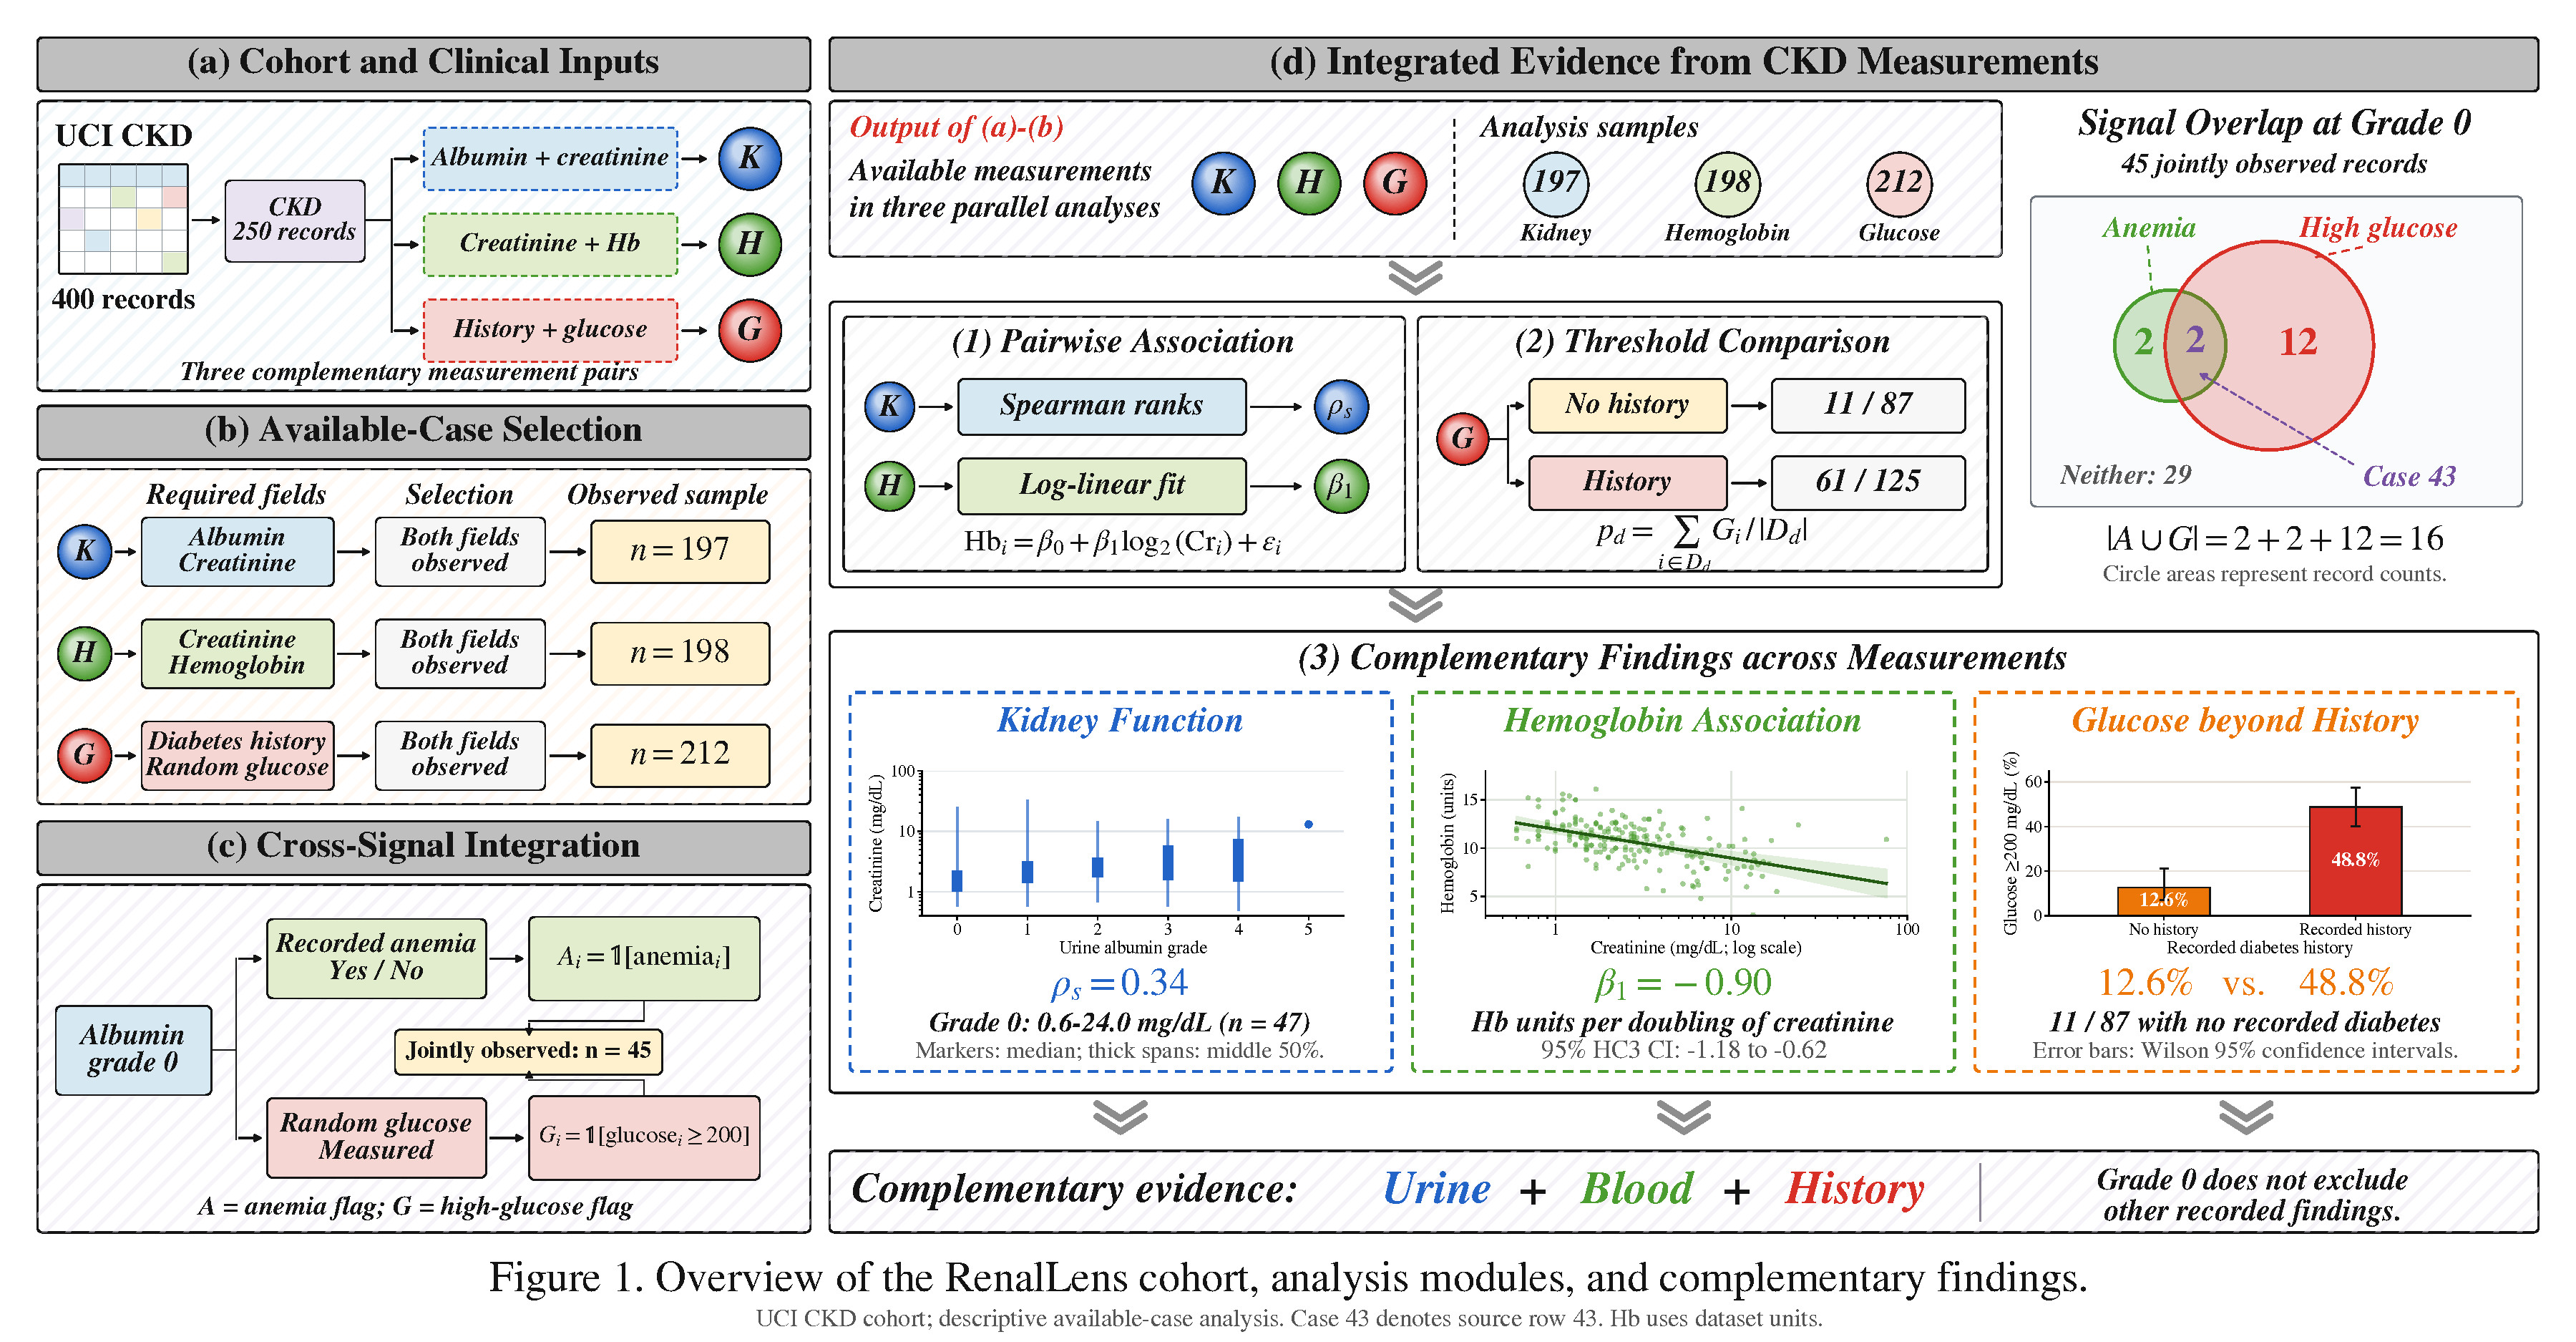
\includegraphics[width=78.5cm]{figures/Figure_1.pdf}};

  \strip{2.5}{60.15}{78.5}{INTERPRETATION AND LIMITATIONS}
  \content{2.5}{61.95}{37.8}{5.65}{{\sz{32}{38}\textbf{\color{red}16 of 45 grade-0 records had anemia, high glucose or both.}\par\vspace{0.25cm}
  Blood measurements added information even when urine albumin was grade 0. Record 43 was one of the two records with both findings.}}
  \draw[grayline,line width=1pt] (41.6,-61.95) -- (41.6,-67.8);
  \content{43.1}{61.95}{37.9}{5.65}{{\sz{30}{36}These cross-sectional hospital records support associations. Missing values change each denominator and may affect comparisons. A random glucose reading alone cannot establish a diagnosis. Hemoglobin retains the dataset's units.}}

  % Right column: record-level anchor and evidence not expanded in Figure 1.
  \strip{82.5}{10.0}{35}{RECORD 43}
  \content{82.5}{11.8}{35}{2.8}{{\sz{32}{38}\textbf{Urine albumin grade 0.}\par No recorded diabetes history.}}
  \ruleat{82.5}{15.15}{35}
  \content{82.65}{15.55}{20}{1.3}{{\sz{32}{38}Blood creatinine}}
  \content{103.0}{15.48}{14.2}{1.3}{{\color{kidney}\bfseries\sz{36}{41}1.0 mg/dL}}
  \ruleat{82.5}{17.05}{35}
  \content{82.65}{17.45}{20}{1.3}{{\sz{32}{38}Hemoglobin}}
  \content{103.0}{17.38}{14.2}{1.3}{{\color{green}\bfseries\sz{36}{41}9.7 units}}
  \ruleat{82.5}{18.95}{35}
  \content{82.65}{19.35}{20}{1.3}{{\sz{32}{38}Recorded anemia}}
  \content{103.0}{19.28}{14.2}{1.3}{{\color{green}\bfseries\sz{36}{41}Yes}}
  \ruleat{82.5}{20.85}{35}
  \content{82.65}{21.25}{20}{1.3}{{\sz{32}{38}Random glucose}}
  \content{103.0}{21.18}{14.2}{1.3}{{\color{red}\bfseries\sz{36}{41}204 mg/dL}}
  \ruleat{82.5}{22.75}{35}
  \content{82.5}{23.15}{35}{1.2}{{\color{muted}\sz{26}{31}Case number identifies the original data row.}}

  \strip{82.5}{25.0}{35}{GLUCOSE AND DIABETES HISTORY}
  \node[anchor=north west,inner sep=0pt] at (82.5,-27.0) {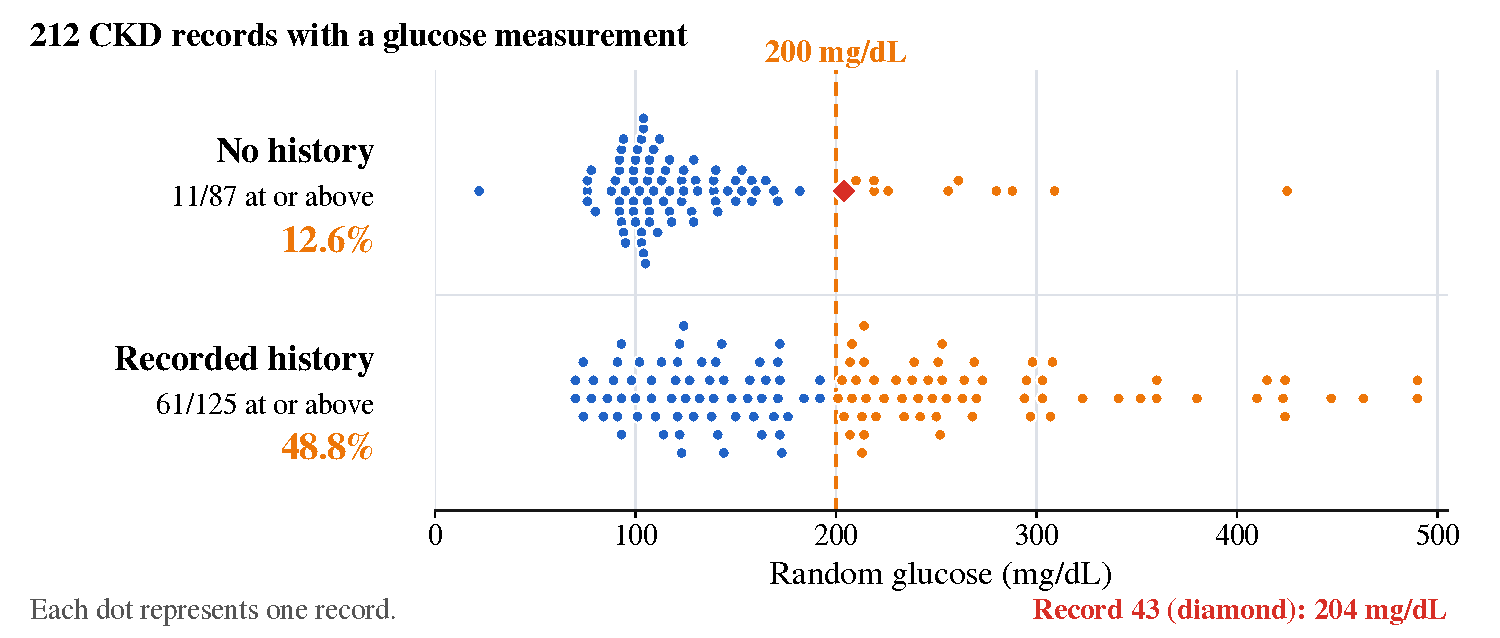
\includegraphics[width=35cm]{figures/Figure_2_Glucose_Distribution.pdf}};
  \content{82.5}{42.45}{35}{2.9}{{\sz{29}{35}\textbf{Figure 2.} Among records without diabetes history, \textcolor{red}{\textbf{11/87 (12.6\%)}} had glucose $\geq200$ mg/dL. Another 38 of all 250 records lacked glucose.}}

  \strip{82.5}{46.25}{35}{CO-OCCURRENCE AND MISSING DATA}
  \node[anchor=north west,inner sep=0pt] at (82.5,-48.1) {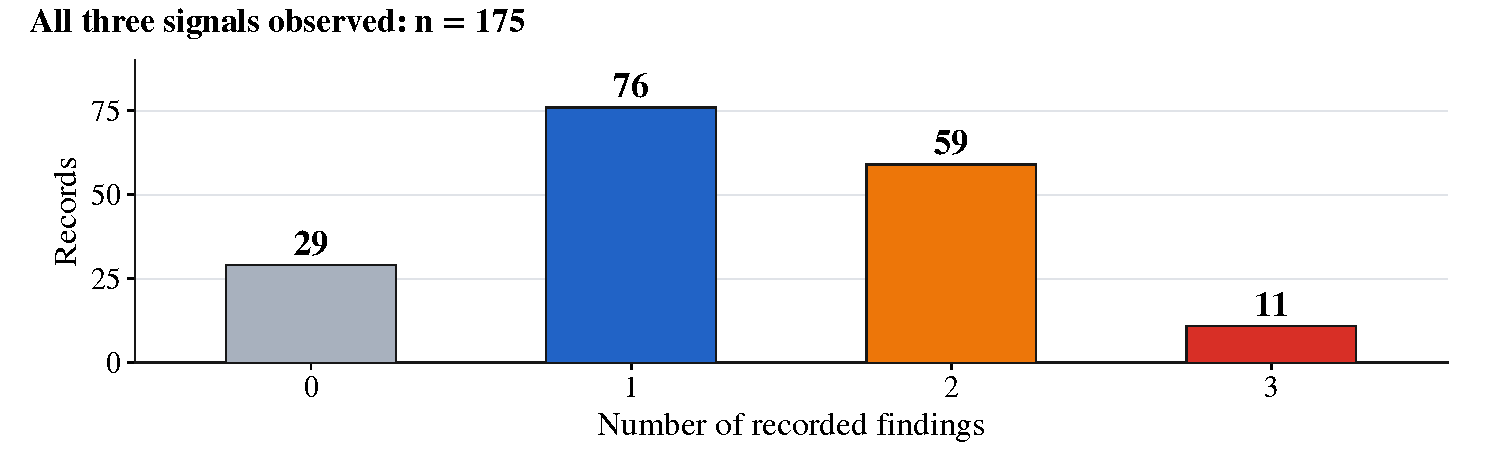
\includegraphics[width=35cm]{figures/Figure_3_Cooccurrence.pdf}};
  \content{82.5}{59.2}{35}{1.5}{{\bfseries\sz{32}{38}\textcolor{red}{70/175 (40.0\%)} had at least two findings.}}
  \node[anchor=north west,inner sep=0pt] at (82.5,-61.0) {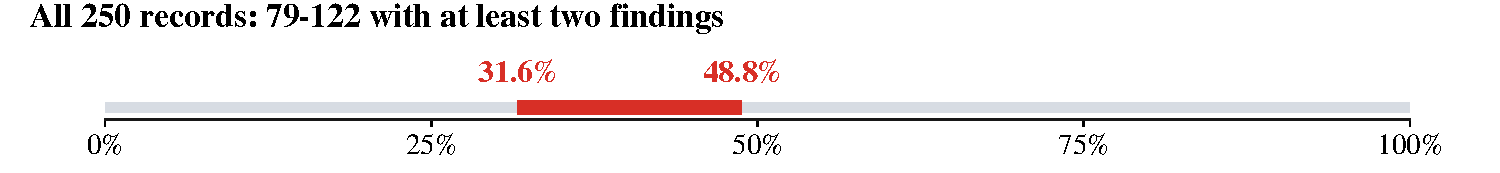
\includegraphics[width=35cm]{figures/Figure_3_Missingness_Bounds.pdf}};
  \content{82.5}{65.05}{35}{2.9}{{\sz{25}{30}\textbf{Figure 3.} Findings: albumin grade $\geq1$, recorded anemia and glucose $\geq200$ mg/dL. Missing results in 75 records give logical bounds of 31.6--48.8\%, rather than a confidence interval.}}

  % Compact provenance remains visible at print size.
  \fill[navy] (0,-69.3) rectangle (120,-72);
  \content{2.5}{69.85}{75}{2.0}{{\color{white}\sz{25}{31}\textbf{Data:} UCI Chronic Kidney Disease (2015), \href{https://doi.org/10.24432/C5G020}{\textcolor{white}{doi:10.24432/C5G020}}.\par
  CKD = chronic kidney disease. All analyses are descriptive and use observed values.\par}}
  \content{82.5}{69.85}{35}{2.0}{{\color{white}\sz{25}{31}\textbf{Project and reproducible analysis}\par
  \href{https://github.com/CanyonChen/RenalLens}{\textcolor{white}{github.com/CanyonChen/RenalLens}}\par}}
\end{scope}
\end{tikzpicture}
\end{document}
